\documentclass{IEEEcsmag}

\usepackage[colorlinks,urlcolor=blue,linkcolor=blue,citecolor=blue]{hyperref}

\usepackage{upmath}
\usepackage{comment}
\usepackage{graphicx}

\usepackage[usenames,dvipsnames,svgnames,table]{xcolor}
\definecolor{dkgreen}{rgb}{0,0.6,0}
\definecolor{mauve}{rgb}{0.58,0,0.82}
\definecolor{light-gray}{gray}{0.88}

\usepackage{listings}
\lstdefinestyle{agree}
{frame=none,
  basicstyle=\ttfamily,
  language=ML,
  aboveskip=3mm,
  belowskip=3mm,
  showstringspaces=false,
  columns=flexible,
  numbers=none,
  numberstyle=\tiny\color{gray},
  commentstyle=\color{dkgreen},
  stringstyle=\color{mauve},
  breaklines=false,
  breakatwhitespace=true,
  tabsize=2,
  linewidth=1.7\linewidth,
  morekeywords={eq, bool, guarantee, assume, true, false, pre, not, and, or, property, const}
}

\newcommand{\briefcase}{BriefCASE}
\newcommand{\hamr}{HAMR}
\newcommand{\selFour}{seL4}
\newcommand{\figref}[1]{Fig.~\ref{#1}}
\newcommand{\agree}{AGREE}
\newcommand{\splat}{SPLAT}
\newcommand{\resolint}{Resolint}
\newcommand{\resolute}{Resolute}

\jvol{XX}
\jnum{XX}
\paper{XX}
\jmonth{XX/XX}
\jname{Security \& Privacy}
\pubyear{2022}
\newtheorem{theorem}{Theorem}
\newtheorem{lemma}{Lemma}

\setcounter{secnumdepth}{0}

\begin{document}

%\sptitle{Department: Head}
%\editor{Editor: Name, xxxx@email}

\title{Cyber Assured Systems Engineering at Scale}

\author{Darren Cofer, Isaac Amundson, Junaid Babar, David Hardin, Konrad Slind}
\affil{Collins Aerospace}

\author{Perry Alexander}
\affil{University of Kansas}

\author{John Hatcliff, Robby}
\affil{Kansas State University}

\author{Gerwin Klein, Corey Lewis}
\affil{University of New South Wales}

\author{Eric Mercer}
\affil{Brigham Young University}

\author{John Shackleton}
\affil{Adventium Labs}

\markboth{Department Head}{Paper title}

\begin{abstract}
Abstract text goes here. This single paragraph ($\le$50 words) summarizes the significant aspects of the manuscript. Often it indicates whether the manuscript is a report of new work, a review or overview, or a combination of thereof. Do not cite references in the abstract. Papers must not have been published previously, must fit into the theme of an open Call for Papers, and must be targeted toward the general technical reader. 
\end{abstract}

\maketitle


\chapterinitial{A rough word count estimate} shows that 1 column in this format is approximately 400 words.  If we start with a budget of 1 column for each section and include two figures and some references, we should come out about right.  

Please add your inputs in separate files.

Darren, David? Budget: 1 column
%Introduction
\chapterinitial{Aerospace systems engineers} are currently given few
development tools to understand and mitigate 
potential cybersecurity vulnerabilities.  Typically, they must rely on
process-oriented checklists and guidelines. Cyber vulnerabilities
are often discovered during penetration testing late in the
development process. Worse yet, they may be discovered
only after the product has been fielded, necessitating extremely
expensive and time-consuming remediation. This is not a
sustainable development model.

Fortunately, formal methods tools have advanced to the point that they can 
be used to address cybersecurity and cyber-resiliency design challenges
on real high-assuance systems at industrial scale.  
Our application domain is avionics and aerospace systems in general.  
They are typically large, real-time cyberphysicial systems with the added 
complexities of performing safety-critical tasks and being exposed to 
a wide variety of cyber threats.  Furthermore, they are subject 
to intense regulatory scrutiny due to the certification requirements of this domain. 

In previous work on the High-Assurance Cyber Military Systems (HACMS) project \cite{HACMS}
we demonstrated that formal methods could be used to dramatically improve the 
cyber-resiliency of real aircraft, including an unmanned military helicopter.  Our current
work is focused on automating the capabilities that we prototyped in the HACMS project
and extending the reach and scale of the formal methods design and verification approach.  

To this end, we have developed a model-based systems engineering (MBSE) 
environment that allows engineers to address a range of properties and 
manage system complexity through compositional analysis, integrating formal methods
at all levels of the design process.  MBSE processes use model as the primary vehicle for 
communication among the parties tasked with designing the system and as the primary 
design artifacts for requirements, verification, and code generation.  

Our tools are based on the 
Architecture Analysis and Design Language (AADL) and extend the Open Source
AADL Tool Environment (OSATE) \cite{OSATE}.  The tools are specifically designed 
to bridge the gap between a user-level modeling language accessible to systems 
engineers and the highly specialized, formally verified code that implements the operating system (OS)
kernel and other high-assurance components.   

By using these tools to build real avionics systems, we show 
that current formal methods tools are practical, effective, and scalable to significant 
high-assurance applications in the aerospace industry.  


\section{INNOVATIONS}
Darren -  Budget: 1 column
%Innovations

MBSE environment for high-assurance systems, providing access to FM tools at every level, integrating assurance evidence for co-evolving design and associated evidence.

\begin{enumerate}
\item Semi-automated architectural design patterns to address cyber-resiliency requirements, including synthesis of high-assurance components
\item MBSE environment that leverages seL4 security guarantees and makes this accessible
\item Co-evolution of system design and certification evidence/artifacts, organized by assurance argument
\item Integration of formal methods throughout the workflow (or is this part of one of the other innovations?)
\end{enumerate}

As part of the DARPA Cyber Assured Systems Engineering (CASE) program,
our team has developed design, analysis, and verification
tools that enable systems engineers to design-in cyber-resiliency
for complex cyber-physical systems. We have produced a prototype
Model-Based Systems Engineering (MBSE) environment called
BriefCASE which is based on the Architecture Analysis and Design
Language (AADL). BriefCASE extends the Open Source AADL
Tool Environmnet (OSATE) to add new design, analysis, and code
generation capabilities targeted at building cyber-resilient systems.
BriefCASE provides access to two analysis tools (GearCASE 
and DCRYPPS) that can examine AADL models to detect potential
cyber vulnerabilities and suggest requirements for mitigation.
A library of architectural transforms guides systems engineers
through automated model transformations that modify the
architecture to address these requirements, possibly inserting new
high-assurance components into the system. Implementations for
these new high-assurance components are synthesized from formal
specifications using the Semantic Properties for Language and
Automata Theory (SPLAT) tool. Formal verification that the
transformed system model satisfies its cyber requirements is accomplished
via model checking using the Assume Guarantee Reasoning
Environment (AGREE). Cyber-resilient code implementing the
verified model is automatically generated using the High Assurance
Modeling and Rapid Engineering for Embedded Systems (HAMR)
toolkit. If desired, this code can be targeted to the formally
verified seL4 secure microkernel.
A novel aspect of our approach is the use of an assurance argument
embedded in the architecture model itself to capture and
document the design decisions made during this process, along
with associated rationale.


\section{EXAMPLE}
Eric?  Budget: 1 column
%Motivation
\begin{figure*}
	\begin{center}
	  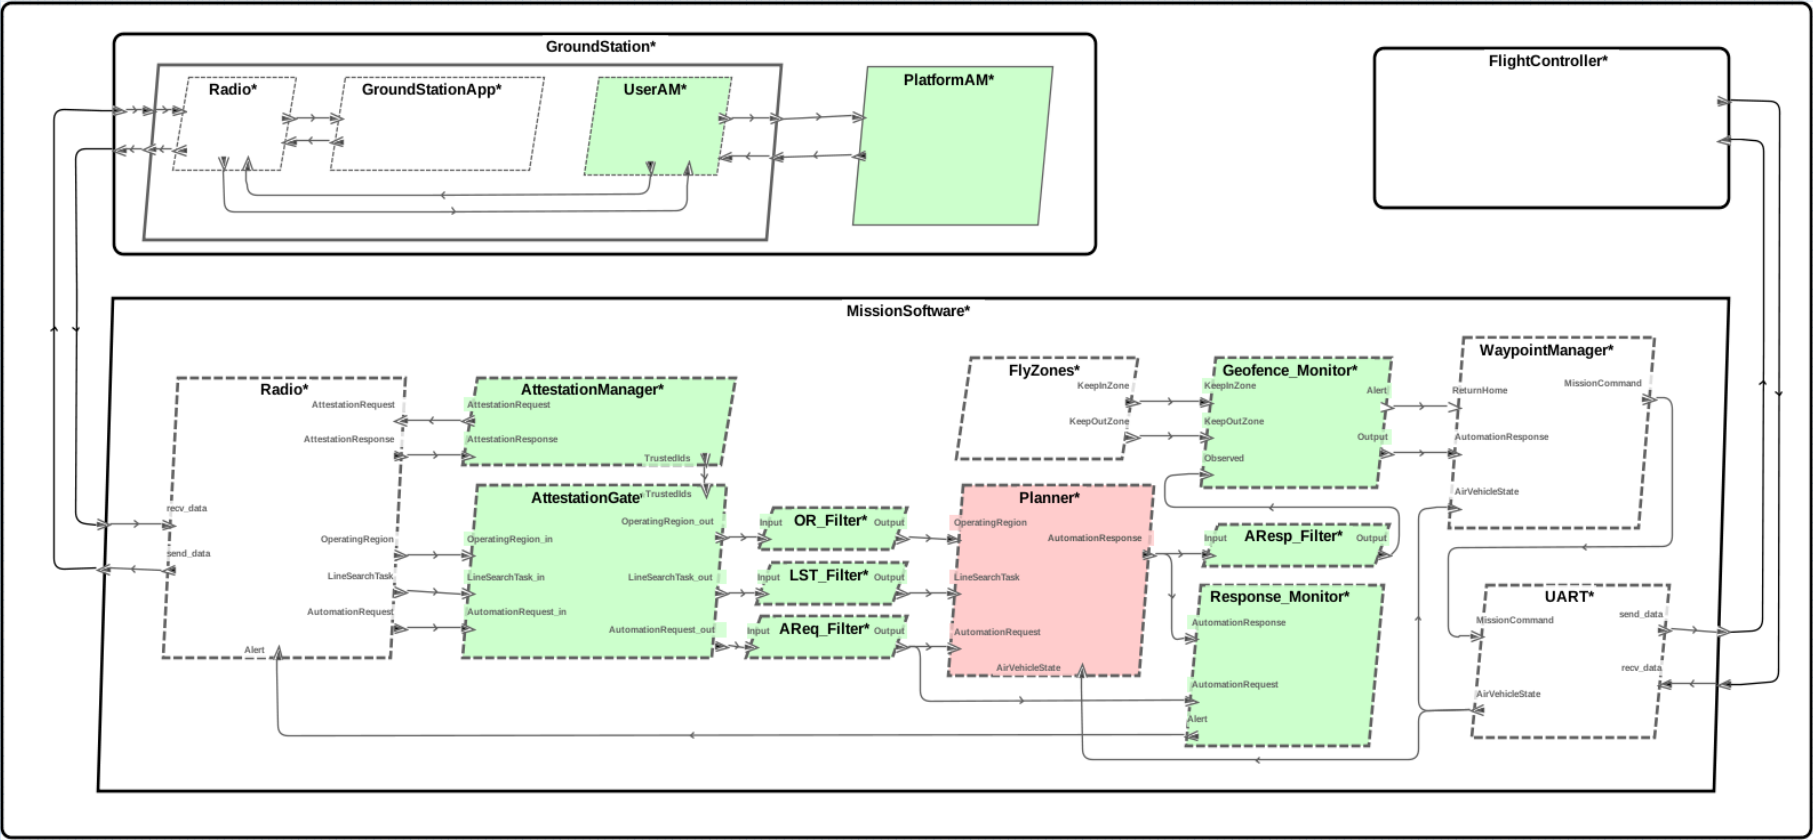
\includegraphics[width=\textwidth]{./figs/sw-hardened.png}
  \end{center}
	\caption{Cyber-resilient software architecture for UAV surveillance system. MAKE NAMES BIGGER} 
	\label{fig:sw-hardened} 
\end{figure*}

\figref{fig:sw-hardened} is a model-based design in the AADL OSATE tool of a cyber-hardened software
system for an autonomous UAV for surveillance.
The original \emph{unhardened system} consists of four components: the radio to communicate with a
remote ground
station (\emph{Radio}), mission planning automation (\emph{UxAS}), waypoint metering
(\emph{WaypointManager}), and a UART to talk to the flight controller (\emph{UART}).

\briefcase\ integrates four key formal methods in the model-based engineering workflow:
assume-guarantee verification (\agree), synthesis of high-assurance components (\splat), synthesis
of inter-component communication (\hamr), and the \selFour\ verified microkernel.
Each component in the unhardened system, and the interface for the top-level software component, is
formally specified with an AGREE contract stating assumptions on inputs and guarantees on outputs
under the assumptions.
\agree\ proves the unhardened implementation obeys the composition of these contracts. 

Cyber-threat analysis (GearCASE and DCRYPPS) identifies the ground station and the planning
automation services as primary cyber threats to the system.
Seven new cyber requirements are added to the unhardened system that require ground station
certification, message integrity, and monitoring.
The existing contracts in the unhardened system are strengthened to reflect these new requirements.
\agree\ proves the unhardened system under these contracts fails verification. 

Design engineers use \briefcase\ to transform the unhardened system to that in
\figref{fig:sw-hardened} by inserting high-assurance components.
\emph{Attestation} proves the identity of trusted ground stations (\emph{AttestationManager}) while
the \emph{gate} only passes messages from trusted sources (\emph{AttestationGate}).
\emph{Filters} only pass well-formed messages (\emph{OR\_Filter}, \emph{LST\_Filter},
\emph{AReg\_Filter}, and \emph{AResl\_Filter}).
\emph{Monitors} alert to suspicious behavior such as missions that enter keep-out zones or leave
keep-in zones (\emph{Geofence\_Monitor}) or unrequested missions from automation
(\emph{Response\_Monitor}).
The interface behavior of these high-assurance components, with the exception of attestation, is
specified with assume-guarantee contracts (e.g., a filter makes no assumptions on input and only
passes input that is well-formed).
\agree\ proves the hardened system ensures the added cyber requirements.

The \selFour\ target platform requires a static schedule that is provided in the model.
A transformation on the \agree\ contracts incorporates that schedule into the verification model.
\agree\ proves the scheduled hardened system also ensures cyber requirements.
The model is further refined to move the attestation and mission planning services into separate
virtual machines inside the microkernel.

\resolint\ certifies the hardened model is ready for synthesis.
\splat\ synthesizes high-assurance components from their \agree\ contracts to the target platform.
It includes proof certificates that the binaries have assumptions that are no stronger than those on
the original contracts and guarantees that are no weaker than those on the original contracts (e.g.,
safe substitution).
\hamr\ synthesizes all the inter-component communication primitives from the AADL model.
That synthesis includes a proof certificate that the resulting communication channels defined in
\selFour\ are only those defined in the AADL model.

\resolute\ builds an assurance case for the entire system.
That assurance case includes evidences for every requirement including proof certificates from
\agree, \splat, and \hamr.


\section{BRIEFCASE WORK FLOW}
Darren right a brief intro -  Budget: 0.5 column
\cite{OSATE}

%Work Flow

%Describe the BriefCASE work flow and tools.

% Copied from DESTION paper
The BriefCASE environment provides systems engineers with a workflow and tool support for developing
products with inherent cyber-resiliency. 
\remove{In this section we provide an overview of the design, analysis, and code generation tools and how they can be used
to implement high-assurance systems.  
}

%BriefCASE is predicated on an MBSE process, in which models are the primary vehicle for
%communication and understanding among the parties tasked with designing the system. Furthermore,
%MBSE models are the primary design artifacts used for analysis, verification, testing, and code
%generation.
The  workflow starts with the development of a baseline AADL model of the system architecture
focusing on the desired functionality. This model can be analyzed using any of the existing AADL 
tools (e.g., resource usage, information flow, latency) to determine whether it is acceptable.
BriefCASE integrates additional tools that analyze the architecture model for cybersecurity vulnerabilities and
generate requirements that, when addressed, will mitigate those vulnerabilities.
These requirements are imported into the model and may be addressed using a 
collection of automated model transforms. As requirements are addressed in the design, an assurance case is updated with
corresponding evidence, computed directly from the model or by supporting analysis tools.  
Code implementing new high-assurance components as well as communication and execution infrastructure
is generated from the model along with associated assurance evidence.  

The following sections describe each step of the workflow in more detail. 

%development process outputs, necessary
%to support the claim. In this manner, the assurance case is co-developed alongside the system
%design, and can be automatically evaluated throughout development.


\subsection{Requirements}
Isaac, Junaid -  Budget: 1 column
\cite{gearcase2020} \cite{dcrypps2019}

BriefCASE provides access to two analysis tools (GearCASE~\cite{gearcase2020} and
DCRYPPS~\cite{dcrypps2019}) that can examine AADL models to detect potential cyber vulnerabilities
and suggest requirements for mitigation.
%
Systems engineers are %then
presented with a requirements management interface
(top pane in Figure~\ref{fig:req-mgmt}) for viewing the generated requirements and importing them into the model
so they can be addressed. The interface enables engineers to select the requirements they wish to
import and assign them unique identifiers, or omit them with rationale. A document listing the omitted
requirements and rationale is maintained and may be a required development artifact for some
certification domains. 

\begin{figure*}[h]
	\centering
	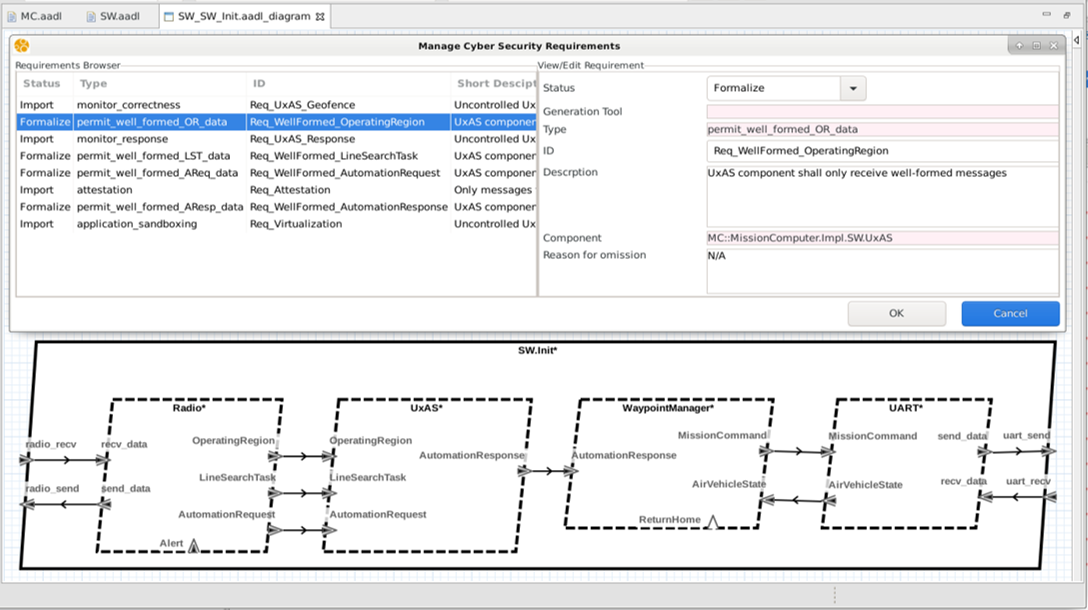
\includegraphics[width=\textwidth]{figs/req-mgmt.png}
	\caption{\briefcase \ requirements management interface.} 
	\label{fig:req-mgmt} 
\end{figure*}

Some requirements can also be formalized as assume-guarantee contracts
added to the AADL model, enabling formal verification. 
Such a requirement will be imported into the model with with an associated formal
contract.

A BriefCASE project contains a repository for requirements. Imported requirements are represented 
as assurance case goals to be satisfied. For example, one of the requirements for well-formed 
messages (selected in \figref{fig:req-mgmt}) is imported as the following goal:

\noindent
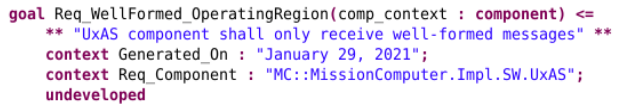
\includegraphics[width=1\columnwidth]{figs/req-wellformed-or.png}

% shown in \figref{fig:req-wellformed-or}.
\noindent
% Initially, the goal is marked {\em undeveloped} and does not contain any evidential statements.  
% These will be added as the design is updated to address this requirement.  
The goal is marked {\em undeveloped} initially.
Evidential statements are added to the goal as
the design is updated to address this requirement.

%for Resolute to evaluate in order to determine whether the goal has been satisfied. Running Resolute
%at this time will therefore produce a failed assurance case.

%\begin{figure}[h]
%	\centering
%	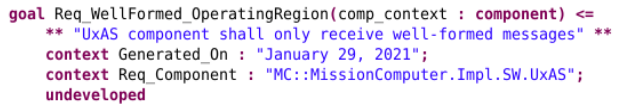
\includegraphics[width=1\columnwidth]{figs/req-wellformed-or.png}
%	\caption{Requirement for well-formed messages.  NEEDED? CONVERT TO TEXT?} 
%	\label{fig:req-wellformed-or} 
%\end{figure}


\subsection{Cyber Transforms}
Isaac -  Budget: 1 column

To address the new requirement, the architecture will need to be transformed in such a way as to harden the design against the vulnerability.
BriefCASE provides a library of model transformations for addressing common cyber vulnerabilities.  Currently, the following transformations are supported:

\begin{itemize}
	\item Attestation
	\item Filter
	\item Monitor
	\item Virtualization
	\item Proxy
	\item Switch
	\item seL4
\end{itemize}  

The transformations are automated by the tool, resulting in a hardened model that is correct-by-construction.  
For example, ensuring a component only receives well-formed messages can be accomplished by the insertion of a high-assurance filter.  The BriefCASE Filter transform wizard (Figure~\ref{fig:filter-wiz}) enables the configuration of filter component properties, including the filter behavioral specification, which is represented in the AGREE language.

\begin{figure}[h]
	\centering
	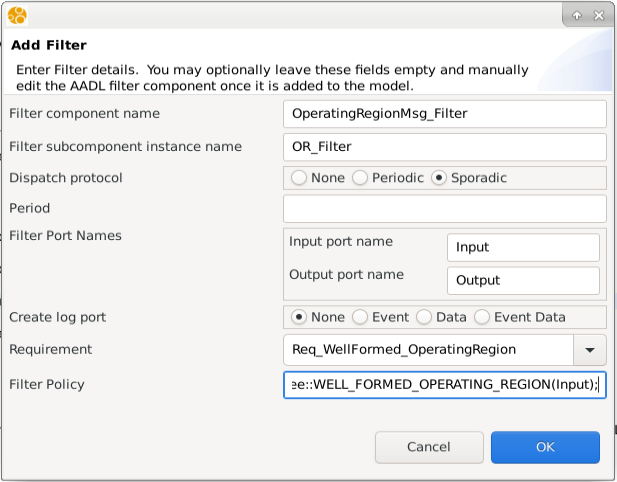
\includegraphics[width=0.7\columnwidth]{figs/filter-wiz.png}
	\caption{Filter transform wizard.} 
	\label{fig:filter-wiz} 
\end{figure}

BriefCASE inserts a new filter component into the model, sets the component properties, and establishes the appropriate connections to source and destination components. The filter specification is inserted into an AGREE annex, enabling both formal analysis of the model as well as providing the behavioral specification for a provably correct synthesis of the component implementation via the SPLAT plugin.

The transformation also updates the Resolute goal with new evidential statements pointing to evidence that the model has indeed been hardened against the vulnerability and the requirement has been satisfied (as shown in Figure~\ref{fig:resolute-add-filter}).
For example, the \texttt{add\_filter} strategy is included in a library of built-in Resolute transform rules and provides Resolute with the logical instructions for evaluating if the top-level goal has been satisfied.
The \texttt{add\_filter} definition (shown in Figure~\ref{fig:resolute-add-filter}) includes the following sub-goals: 
\begin{itemize}
	\item \texttt{filter\_exists} - the filter component exists in the model
	\item \texttt{filter\_not\_bypassed} -  there is no alternate pathway in the model that can bypass the filter
	\item \texttt{filter\_implemented\_correctly} - the filter has been implemented correctly
\end{itemize}


\begin{figure}[h]
	\centering
	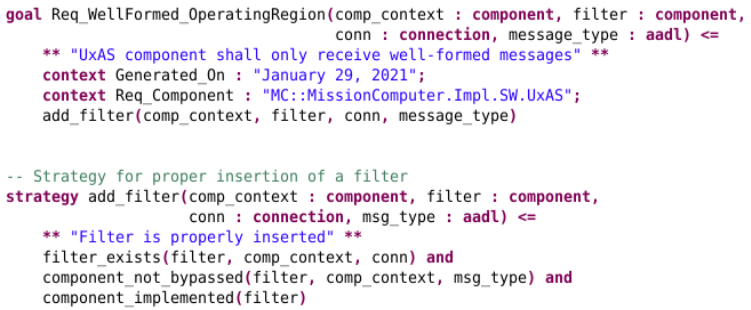
\includegraphics[width=1\columnwidth]{figs/resolute-add-filter.png}
	\caption{Updated well-formedness claim.} 
	\label{fig:resolute-add-filter} 
\end{figure}

The first two sub-goals are supported by evidence obtained by examining the structure of the model, while the last is determined by examining the output of the synthesis tool.  This approach follows the model-based decomposition pattern based on~\cite{model-based-decomposition}, and is representative of all BriefCASE transform assurance strategies.
If at a later time during development the model is inadvertently altered in a way that renders the transformation ineffective, Resolute will be unable to substantiate the evidential statements, and therefore produce a failing assurance case.

The third subgoal is satisfied by SPLAT.  SPLAT not only generates the  implementation code for high-assurance components such as filters, monitors, and gates, but it also produces a proof that this code correctly implements its AGREE specification.  
Resolute uses the existence of the SPLAT proof as evidence that the component was implemented correctly.

\subsection{High Assurance Component Synthesis}
Konrad, Eric, Junaid -  Budget: 1 column
\cite{case-verified-filter} \cite{hardin-co-assurance}
\cite{formal-filter-synth-langsec} \cite{contiguity-types} 

\subsection{Remote Attestation}
Perry -  Budget: 1 column
\cite{copland-attestation} \cite{copland-verification}

\subsection{Compositional Analysis}
Isaac, Junaid -  Budget: 1 column
\cite{case-models-2021}

\subsection{Information Flow Analysis}
John H -  Budget: 1 column

\subsection{Real-Time Scheduling}
John S -  Budget: 1 column

\subsection{Infrastructure Code Generation}
John H -  Budget: 1 column

\subsection{Secure Microkernel}
Corey, Gerwin -  Budget: 1 column
\cite{sel4-formal}

\subsection{Assurance Case}
Isaac -  Budget: 1 column
\cite{resolute-destion}

An important aspect of our work on CASE has been to structure formalizations and proofs by following the AADL description of the system. In other work, we did this through the use of formal assume-guarantee contracts that correspond to the requirements for each component~\cite{HACMS}. We have found that in assuring the cyber-security properties of aircraft designs we need to integrate different kinds of evidence with varying levels of formality. This has been our motivation to explore assurance case methods.

In previous work, we developed the {\em Resolute} language and tool~\cite{resolute2014},~\cite{resolute-destion} as a way to help developers create an assurance argument describing the steps taken during the design process to make the system safe and secure.  
The Resolute syntax supports construction of assurance cases that comply with the Goal Structuring Notation (GSN) v2 standard~\cite{GSNv2}.  Claims are expressed as \textit{goals} and \textit{strategies}, and can contain attributes such as \textit{context}, \textit{assumptions}, and \textit{justification}.  Claims can be marked \textit{undeveloped}, which Resolute interprets as an unsupported claim, or with a \textit{solution}, which is an explicit assertion that the claim is supported.
Rather than being a separate document, a Resolute assurance case is part of the architecture model and can refer to elements within the model. Since it is not a static representation, it can ensure that the assurance argument remains consistent with the evolving design.

BriefCASE includes a library of Resolute assurance strategies, or \textit{patterns}, that align with the CASE workflow.  The patterns are instantiated with context from the AADL model, and specify the evidence required to support the cyber-resiliency goals of the system.  
%
For example, the \texttt{add\_filter} strategy is automatically inserted into the assurance case when the \textit{Filter} transformation is performed, and includes logical rules that Resolute uses to determine whether the well-formedness claim is  supported by evidence.
The \texttt{add\_filter} definition (shown in Figure~\ref{fig:resolute-add-filter}) includes the following sub-goals: 
\begin{itemize}
	\item \texttt{filter\_exists} - the filter component exists in the model
	\item \texttt{filter\_not\_bypassed} -  there is no alternate pathway in the model that can bypass the filter
	\item \texttt{filter\_implemented\_correctly} - the filter has been implemented correctly
\end{itemize}


\begin{figure}[h]
	\centering
	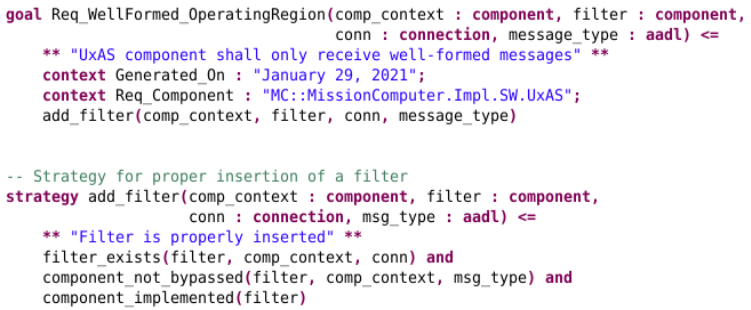
\includegraphics[width=1\columnwidth]{figs/resolute-add-filter.png}
	\caption{Updated well-formedness claim.} 
	\label{fig:resolute-add-filter} 
\end{figure}

The first two sub-goals are supported by evidence obtained by examining the structure of the model, while the last is determined by examining the output of the synthesis tool.  
If at a later time during development the model is inadvertently altered in a way that renders the transformation ineffective, Resolute will be unable to substantiate the evidential statements, and therefore produce a failing assurance case.

The third subgoal is satisfied by SPLAT.  SPLAT not only generates the implementation code for high-assurance components such as filters, monitors, and gates, but it also produces a proof that the generated code correctly implements its AGREE specification.  
Resolute uses the existence of the SPLAT proof as evidence that the component was implemented correctly.


% Resolute can determine whether an assurance case passes or fails


% Advocate?

% Show generated assurance case (in Advocate?)

\section{AIRCRAFT APPLICATION}
David -  Budget: 1 column

Describe how we have used the BriefCASE tools to add new functionality to the CAAS architecture.  

\section{CONCLUSION}
 Budget: 0.5 column
The manuscript should include a conclusion. In this section, summarize what was described in your paper. Future directions may also be included in this section. Authors are strongly encouraged not to reference multiple figures or tables in the conclusion; these should be referenced in the body of the paper.

\section{ACKNOWLEDGMENT}

This work was funded by DARPA contract HR00111890001. The
views, opinions and/or findings expressed are those of the author
and should not be interpreted as representing the official views or
policies of the Department of Defense or the U.S. Government.

\bibliographystyle{IEEEtran}
\bibliography{biblio}

\begin{IEEEbiography}{Darren Cofer}{\,}is a Fellow at Collins Aerospace. His research interests include formal methods and tools for verification and certification of high-integrity systems. He received his PhD in Electrical and Computer Engineering from the University of Texas at Austin and is a senior member of the IEEE. Contact him at cofer@ieee.org.
\end{IEEEbiography}

\begin{IEEEbiography}{Isaac Amundson}{\,}is a research engineer at Collins Aerospace, focusing on MBSE, formal verification and assurance.  He received his PhD in Computer Science from Vanderbilt University.
\end{IEEEbiography}

\begin{IEEEbiography}{Junaid Babar}{\,}is a researcher at Collins Aerospace.
Do not fold, spindle, or mutilate.  
\end{IEEEbiography}

\begin{IEEEbiography}{David Hardin}{\,}is a research engineer
  at Collins Aerospace, and has made contributions in
  the areas of formal methods, high-assurance computer architecture,
  and real-time embedded Java.  He is editor of the book \emph{Design
    and Verification of Microprocessor Systems for High-Assurance
    Applications}.  He received a PhD in Electrical and Computer
  Engineering from Kansas State University.
\end{IEEEbiography}

\begin{IEEEbiography}{Konrad Slind}{\,} (PhD, TU Munich) is an industrial logician at Collins Aerospace.
  His research interests include design and implementation of higher
  order logic theorem provers, verified compilation, and
  self-describing data formats.
\end{IEEEbiography}

\begin{IEEEbiography}{Perry Alexander}{\,}is the AT\&T Foundation
  Distinguished Professor and Director of The Information and
  Telecommunication Technology Center at The University of Kansas.
  His research interests include trusted computing, remote
  attestation, formal verification and formal synthesis. He received
  his PhD from The University of Kansas.
\end{IEEEbiography}

\begin{IEEEbiography}{John Hatcliff}{\,}
John Hatcliff is a University Distinguished Professor and
Lucas-Rathbone Professor of Engineering in the Computer Science
Department at Kansas State University.  His research interests include
software architecture, formal verification, and interoperability in 
the avionics, automotive, and medical domains.
He received his PhD in Computer Science from Kansas State University.
\end{IEEEbiography}

\begin{IEEEbiography}{Robby}{\,}
is a Professor of Computer Science at Kansas State University working
in the area of formal methods, software engineering, and programming
languages.
%%He received his PhD in Computer Science from Kansas State University.
He received a NASA Turning Goals Into Reality award in 2003,
a NSF CAREER award in 2007, an ICSE 2000 Most Influential Paper award in 2010,
and an ACM SIGSOFT Impact award in 2010.
\end{IEEEbiography}

\begin{IEEEbiography}{Gerwin Klein}{\,}
is Chief Scientist at Proofcraft and Conjoint Professor at UNSW Sydney. His
research interests include software verification, semantics of programming
languages, and proof engineering. He is the architect of the seL4 microkernel
verification which received the SIGOPS Hall of Fame Award. He received his PhD
in Computer Science from TU Munich.
\end{IEEEbiography}

\begin{IEEEbiography}{Corey Lewis}{\,}%
  is a Senior Proof Engineer at UNSW Sydney. He has been involved in all stages
  of the verification of the seL4 microkernel.
\end{IEEEbiography}

\begin{IEEEbiography}{Eric Mercer}{\,}
  is an Associate Professor at Brigham Young University.
  His research interests include software verification, model checking, static analysis, and programming languages.
  He received his PhD in Electrical Engineering from the University of Utah.
\end{IEEEbiography}

\begin{IEEEbiography}{John Shackleton}{\,}
  is a Senior Principal Research Scientist at Adventium Labs,
  focused on real-time embedded systems, cybersecurity, and
  model-based system engineering and analysis.
\end{IEEEbiography}

%Author's latest degree received or which he/she is currently pursuing
%(He received the B.S. degree and the M.S. degree...."). Author's
%research interest. Association with any official journals or
%conferences; major professional and/or academic achievements, i.e.,
%best paper awards, research grants, etc.; any publication information
%(number of papers and titles of books published). Author membership
%information, e.g., is a member of the IEEE and the IEEE Computer
%Society, if applicable, is noted at the end of the
%biography. Biography is limited to single paragraph only (He is a
%member of IEEE, etc.). All biographies should be limited to one
%paragraph, five to six sentences


\end{document}

